\documentclass{article}
\usepackage{amsmath, amssymb, tikz, geometry, graphicx, natbib, mwe, xcolor,
 listings, tabularx, pdfpages, blindtext, mathtools, stackengine, amsthm, pgfplots,bigints, relsize, upgreek, esint, array, multirow}
\usepackage{hyperref}
\usepackage{slashed, enumitem}

\pgfplotsset{width=10cm,compat=1.9}

\colorlet{myWhite}{white!35!gray}
\definecolor{shadeofgray}{HTML}{181818}
\definecolor{shadeofviolet}{HTML}{0f022c}

\hypersetup{
    colorlinks=true,
    linkcolor=violet,
    filecolor=magenta,      
    urlcolor=cyan,
    pdftitle={Overleaf Example},
    pdfpagemode=FullScreen,
}

\geometry{ 
 a4paper,
 total={170mm,257mm},
 left=20mm,
 top=10mm,
 }
 
\lstdefinestyle{mystyle}{ 
bracketsstyle=\color{red}
}

\DeclareMathOperator{\sgn}{\text{sgn}}

\title{Formulario di Fondamenti di Telecomunicazioni}
\author{Giuseppe Bumma}


%----------------------------------------------------------------------
%use this for a total black background
%\pagecolor{black}
%\color{myWhite}
%----------------------------------------------------------------------


\pagecolor{shadeofgray}
\color{myWhite}



\begin{document}

%Commands
\newcommand{\R}{\mathbb{R}}
\newcommand{\bb}[1]{\mathbb{#1}}
\newcommand{\cc}[1]{\mathcal{#1}}
\newcommand{ \lognormal }{\text{Lognormal} }
\newcommand{\tb}[1]{\textbf{#1}}
\newcommand*\circled[1]{\tikz[baseline=(char.base)]{%
            \node[shape=circle,draw,inner sep=2pt] (char) {#1};}}
%for using circled number in enumerate use:
%\begin{enumerate}[label=\protect\circled{\arabic*}]


\tableofcontents

\maketitle

\section{Numeri complessi}
\begin{center}
    \renewcommand{\arraystretch}{2.5}
    \begin{tabular}{c c}
        Unità immaginaria & $j^2=-1$\\
    \end{tabular}
    \begin{tabular}{c c}
        Forma classica & $z = a + jb$\\
    \end{tabular}
\end{center}
\subsubsection*{Coordinate Polari}
\begin{align*}
    a &= r \cos(\phi) & r &= \sqrt{a^2 + b^2}\\
    b &= r \sin (\phi) & \phi &= 
    \begin{cases}
        \arctan\left( \dfrac{b}{a} \right) &a > 0\\
        \\
        \sgn(y) \cdot \dfrac{\pi}{2} &x=0\\
        \\
        \arctan \left( \dfrac{b}{a} \right) + \pi &a<0
    \end{cases}
\end{align*}
\subsubsection*{}


\subsubsection*{Forma esponenziale}
\begin{align*}
    e^{j \phi} &= \cos(\phi) + j \sin(\phi) & z&= a + jb = r e^{j \phi} 
\end{align*}
\begin{center}
    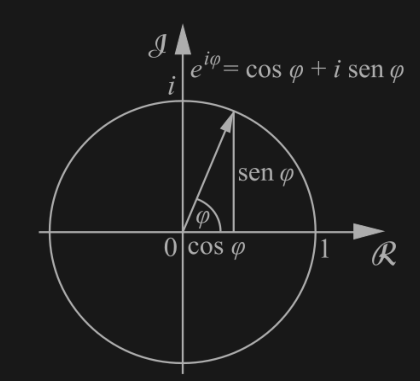
\includegraphics[scale=0.5]{Circonferenza.png}
\end{center}




\section{Sinusoide e fasori}
\renewcommand{\arraystretch}{2.5}
\begin{center}
    \begin{tabular}{|c|c|}
        \hline
        Funzione sinusoidale & $x(t) = A \cos (\omega t + \theta) = Re \left\{  A e^{j(\omega t + \theta)}\right\}$\\
        \hline
    \end{tabular} 
\end{center}


\subsection{Analisi di Fourier}
\begin{center}
    \renewcommand{\arraystretch}{3}
    \begin{tabular}{|c|l|}
        \hline 
        \multirow{2}{7em}{Prima forma (esponenziale)} & formula di sintesi: $x(t)=\mathlarger{\sum}_{n=-\infty}^{+\infty} c_n e^{jn \omega_0t}$\\
        & formula di analisi: $c_n = \dfrac{1}{T} \bigintss_{-T/2}^{+T/2} x(t)e^{-jn\omega_0t}dt$\\
        \hline
        Convergenza puntuale & $\lim\limits_{N \rightarrow \infty} \left\{ x(t) - \mathlarger{\sum}_{n=-N}^N c_n e^{jn\omega_0t} \right\}=0$\\
        \hline
        Convergenza in media quadratica & $\lim\limits_{N \rightarrow \infty} \left\{ \bigintss_T \left| x(t) - \mathlarger{\sum}_{n=-N}^N c_n e^{-jn\omega_0t} \right|^2 dt \right\}=0$\\
        \hline
        $I^o$ forma serie di Fourier & $x(t) =c_0 + \mathlarger{\sum}\limits_{n=1}^{+\infty} Re \left\{ 2c_n e^{jn\omega_0t} \right\} $\\
        \hline 
        \multirow{3}{*}{$II^o$ forma serie di Fourier} & 
        \begin{tabular}{l l}
            $A_o = c_0$ & $\phi_n = - arg \{c_n\}$\\
            $A_n = 2 |c_n|$\\
            $x(t) = A_0 + \mathlarger{\sum}_{n=1}^{+ \infty} A_n \cos (n\omega_0 t - \phi_n)$\\
        \end{tabular}\\
        \hline
        \multirow{3}{*}{$III^o$ forma serie di Fourier} & 
        \begin{tabular}{l l}
            $a_o = 2c_0$ & $b_n = - I_m \{2c_n\}$\\
            $a_n = Re \{2 c_n \}$\\
            $x(t) = \dfrac{1}{2} a_0 + \mathlarger{\sum}_{n=1}^{+ \infty} a_n \cos(n\omega_0t) + \mathlarger{\sum}_{n=1}^{+ \infty}b_n \sin(n\omega_0t)$
        \end{tabular}\\
        \hline
    \end{tabular}
\end{center}


\subsection{Trasformata e integrale di Fourier}
\begin{center}
    \renewcommand{\arraystretch}{3}
    \begin{tabular}{|c|l|}
        \hline
        Formula di Analisi & $ X(\omega) = \bigintss_{-\infty}^{\infty} x(t)e^{-j\omega t} \ dt$\\
        \hline
        Formula di sintesi (\textbf{antitrasformata}) & $ x(t) = \dfrac{1}{2 \pi} \bigintss _{- \infty}^{+ \infty} X(\omega) e^{j \omega t} \ d\omega $\\
        \hline
        Spettro di ampiezza monolatero & $ V(\omega) = \dfrac{|X(\omega)|}{\pi} \ \ \omega \geq 0$\\
        \hline
        Integrale di Fourier (solo se $x(t)\in \R$) & $ x(t) = \bigintss_{0}^{+ \infty} V(\omega) \cos[\omega t - \phi(\omega) ] \ d \omega $\\
        \hline
        \multirow{2}{*}{Proprità trasformata di Fourier} & Coniugazione: $F[x^*(t)] = X^*(-\omega) $\\
        &Traslazione temporale: $F[x(t - t=o)] = X(\omega) e^{-j\omega t_0} $\\
        & Derivata: $F[\dot x(t)] = j \omega X(\omega)$\\
        & Integrale: $F \left[ \bigintss_{- \infty}^{t} x(\xi) \ d\xi \right] = \dfrac{X(\omega)}{j\omega}$ se $X(0) = \left[ \bigintss _{- \infty}^{+ \infty} x(t) \ dt \right] = 0 $\\
        & Convoluzione:\\
        &\begin{tabular}{l}
            $x(t) \cdot y(t) = \bigintss_{- \infty}^{+ \infty} x(\tau) y(t - \tau) \ d\tau \Longrightarrow$ \\
            $F [x(t) \cdot y(t)] = X(\omega)Y(\omega)$
        \end{tabular}\\
        \hline   
    \end{tabular}
\end{center}


































\end{document}